\documentclass[conference]{IEEEtran}
\IEEEoverridecommandlockouts
% The preceding line is only needed to identify funding in the first footnote. If that is unneeded, please comment it out.
\usepackage{cite}
\usepackage{amsmath,amssymb,amsfonts}
\usepackage{algorithmic}
\usepackage{graphicx}
\usepackage{textcomp}
\usepackage{xcolor}
\usepackage{tabularx}
\usepackage{graphicx}
\graphicspath{ {./images/} }
\usepackage{listings}
\def\BibTeX{{\rm B\kern-.05em{\sc i\kern-.025em b}\kern-.08em
\kern-.1667em\lower.7ex\hbox{E}\kern-.125emX}}
\begin{document}

%This is the title, add edits inside {}
\title{DDoS Mitigation in 5G
DAWN: Distributed and Adaptive Workflow Network
}
% author - add 
\author{\IEEEauthorblockN{ Lalli, Aisha | Tripathi, Arti | Sanapala, Madhu}
\IEEEauthorblockA{
\textit{New York University}  (Tandon School of Engineering), New York, USA}
}
\maketitle 
%\section{Abstract}
\begin{abstract} 
This paper delves into the security challenges that 5G networks endure when faced with Distributed Denial of Service (DDoS) attacks. After conducting a thorough review of existing protective solutions and measures, we introduce a novel network architecture, the Distributed Adaptive Workflow Network (DAWN). Positioned at the edge of the core network, DAWN offers  protection to vital servers. DAWN leverages the capabilities of machine learning, SDN, and NFV architectures. It also uses the capabilities of whitelisting and hardware and virtual preprocessors to neutralize incoming DDoS attacks. Using comprehensive literature reviews and theoretical explorations, we advocate that DAWN is potentially a groundbreaking guard against DDoS attacks in the evolving 5G era.  We conclude with recommendations for future research and development in bolstering network security. 

Video Presentation - https://stream.nyu.edu/id/1\_gzfe3lul
Github - https://github.com/allali7/DAWN-SDN

\textbf{Keywords— DAWN, CISCO Guard, AKMAI Kona, DDoS, 5G, Network Security}
\end{abstract}

\section{Introduction}
The advent of 5G networks signifies a monumental leap in wireless communication technology, featuring remarkable improvements in connectivity, data transmission speeds, and the ability to accommodate a diverse range of innovative applications. However, with the complexity of these advanced networks, the vulnerability to cyber threats, particularly Distributed Denial of Service (DDoS) attacks, has notably increased [16]. DDoS attacks exploit network protocols and are more notably orchestrated to overwhelm and disrupt network services by bombarding them with an excessively high volume of internet traffic. The attacks, which can be launched on different network segments including the edge, core, and multi-domain, cause an exponential increase in the traffic directed at the victim's network [4]. The server's processing capacity and bandwidth subsequently become overwhelmed, resulting in slow, unresponsive, or completely inaccessible services to legitimate users. As 5G gets more heavily implemented with our network infrastructure, Enhanced Mobile Broadband (eMBB) and Massive Machine-Type Communications (mMTC) which support faster connections can be used to send large volumes of data ensuing a debilitating attack on the entities targeted. This is an overwhelming challenge for security professionals, which needs a high capacity and flexible solution. Our research will explore an innovative solution, compare existing solutions, and conclude with an analysis of our findings [4][16][11][17]. 

%%%% ADD THESE ARE THE FOLLOWING SECTIONS
%%% NOTE FOR WHY THIS IS SO LONG
%% THE FOLLOWING SECTIONS WILL BE
%% BOLD SECTION TITles

\section{Background}
In the domain of 5G, the ubiquity of internet-connected devices increases the feasibility of DDoS attacks. The relative novelty of 5G also introduces unknown vulnerabilities that hackers may exploit. The integration of 5G technologies further complicates the fight against DDoS attacks, as the network architecture differs significantly from earlier generations, making traditional countermeasures potentially ineffective. With the advent of 5G, important considerations such as the broad array of services and devices, the high speed and low latency that could potentially flood a network more swiftly, and the implications of edge computing, where data is stored and processed at numerous locations, thus increasing the surface area for an attack, becomes pivotal.

Notably, we have explored three main research papers that have tackled the problem of DDoS in 5G by focusing on distinct segments of the network. The first paper addresses vulnerabilities in Software Defined Networks (SDNs), proposing machine-learning approaches for attack prediction [10]. The second paper proposes an implementation of NIDS (Network Intrusion Detection Systems) plus an alert enhancer to capture and parse inner headers for edge, core, and multi-domain segments [4]. Lastly, the third paper suggests algorithms for resource monitoring and load balancing to counter base station attacks [18].

Despite the considerable contributions made by these research papers and others in the security community, DDoS attacks in 5G networks remain a formidable challenge. Many of these solutions focus on small software, but the problem will remain if hardware issues are not addressed. The rapidly evolving nature of the problem, coupled with the technical and economic constraints in combating such attacks, demands fresh and innovative solutions that can effectively tackle these unique challenges and complexities. 

To this end, we propose a new network architecture, the Distributed Adaptive Workflow Network (DAWN), that can potentially provide an effective defense against DDoS attacks. However, our proposed solution is theoretical and cannot be empirically tested at this stage. Therefore, its effectiveness and potential shortcomings will be assessed based on the analysis of other works in the field. We will delve into the examination of areas including load-balancing algorithms, machine learning-based attack indicators, existing solutions, and resilience strategies. We will also discuss the roles of SDN and NFV architectures, whitelisting techniques, edge networks within 5G, hardware and virtual preprocessors' capabilities, and conduct a cost-benefit analysis for DDoS impacts versus DAWN implementation.

The 2021 DDoS attack on VOIP.ms underscores the urgency of advanced cybersecurity solutions like DAWN (Dynamic Analysis and Warning Network) in the 5G landscape. This event exposed the vulnerability of VoIP services, disrupting over 80,000 customers across 125 countries and demanding a substantial ransom, showcasing the escalating trend of financial exploitation through DDoS attacks [2]. DAWN's integration of AI, SDN, NFV, and hardware preprocessors could have dynamically mitigated the attack, bridging the gap in countering evolving threats within 5G networks [6].
The stakeholders for DAWN encompass organizations heavily reliant on digital communication systems, including businesses operating VoIP services, financial institutions, healthcare providers, and government agencies. The susceptibility of services like VoIP to DDoS attacks highlights the immediate need for solutions like DAWN, offering proactive protection to ensure uninterrupted services and financial resilience. Moreover, DAWN's SDN architecture offers an ideal solution for safeguarding specialized servers that require continuous operation, providing an extra layer of protection without compromising functionality. 


\section{OVERVIEW OF THEORETICAL STRATEGY } 

According to Lohachab et al. “more intelligent systems should be developed by utilizing technologies, such as artificial intelligence, machine learning, SDN, and network function virtualization in order to deal with novel DDoS attacks” [1]. Our hypothesis suggests that DAWN, a system of core edge-located hardware preprocessors controlled by an alert-activated Software Defined Network (SDN), which remains idle until activated by a DDoS alert, can provide an effective, scalable, and dynamic defense against DDoS attacks in large-scale networks, particularly in the context of 5G. This alert-driven activation of the DAWN SDN reduces unnecessary overhead and strain on network resources during normal operation while enabling a rapid response during attack scenarios. DAWN, acting as a distributed shield, will process and filter inbound traffic at the core network's edge, whitelisting legitimate packets and black-lisiting malicious ones. DAWN uses the power of SDN and NFV, to awaken the necessary number of hardware preprocessors to filter the traffic whilst each hardware preprocessor uses threads of virtual preprocessors as well. As a result, regular server operations will be protected, and the primary SDN will experience significantly reduced strain, as DAWN will manage the majority of the attack traffic away from the network's core. Despite its higher initial costs, DAWN incorporates a fallback mechanism to conventional load balancing in the event of an SDN failure, enhancing network resilience, and making it a potentially viable solution for enhancing network security in an era of increasingly sophisticated DDoS threats.

\section{DAWN: AN ALERT-ACTIVATED SDN} 
Concept and architecture of DAWN
The architecture of DAWN is built around a DAWN Software Defined Network (SDN) linked to dedicated servers, termed DAWN preprocessors. As a 5G solution, DAWN's SDN is also connected to the client's network SDN, necessitating an SDN-based network. This forms the architectural function of DAWN, where the DAWN SDN serves as a dynamic traffic manager, the Preprocessors as the inspectors, and the main SDN as the primary handler. 

 DAWN was conceived with the primary goal of safeguarding crucial servers from potential attacks. Upon detecting a possible attack by the target server or main SDN, the main SDN dispatches an alert to the DAWN SDN. This action triggers traffic redirection from the target server(s) to the DAWN SDN, isolating potentially malicious traffic, and the regular workflow is not interrupted or permeated. The DAWN system thus serves as an emergency buffer, activating the physical preprocessors solely during attacks. The primary and necessary objective is to offload attacks from critical servers, ensuring uninterrupted client services.

Upon receiving an alert, the DAWN SDN assesses traffic volume and distributes the load accordingly across a calculated number of physical servers. This dynamic activation of more preprocessors showcases DAWN's scalability and flexibility. It employs threading to establish virtual preprocessors within each physical preprocessor, thus augmenting processing speed to cope with the incoming traffic. 

In order to preserve integrity, the preprocessors scrutinize incoming packets using a defense algorithm and categorize them as either whitelisted or blacklisted, with each category assigned an appropriate time-to-live duration. More comprehensive details of the defense algorithm will be covered in subsequent sections. 

Upon receiving these lists, the DAWN SDN circulates them among the preprocessors and updates the main SDN. If the DAWN SDN is directly targeted, the server preprocessor could still manage load balancing and filtering using Network Function Virtualization (NFV) functionalities providing flexibility in recalibrating its defense strategy when needed. Though this setup would not be as robust as having an active DAWN SDN, the system needs to withstand multiple targeted attacks and prevent single points of failure.

Post-attack, the DAWN SDN deactivates all operational preprocessors and reverts to an idle state. Although DAWN can be deployed as a singular defensive strategy, it can also be configured as a distributed system for larger network protection, thereby adding an additional layer of resilience to the network.


\begin{figure}[h]
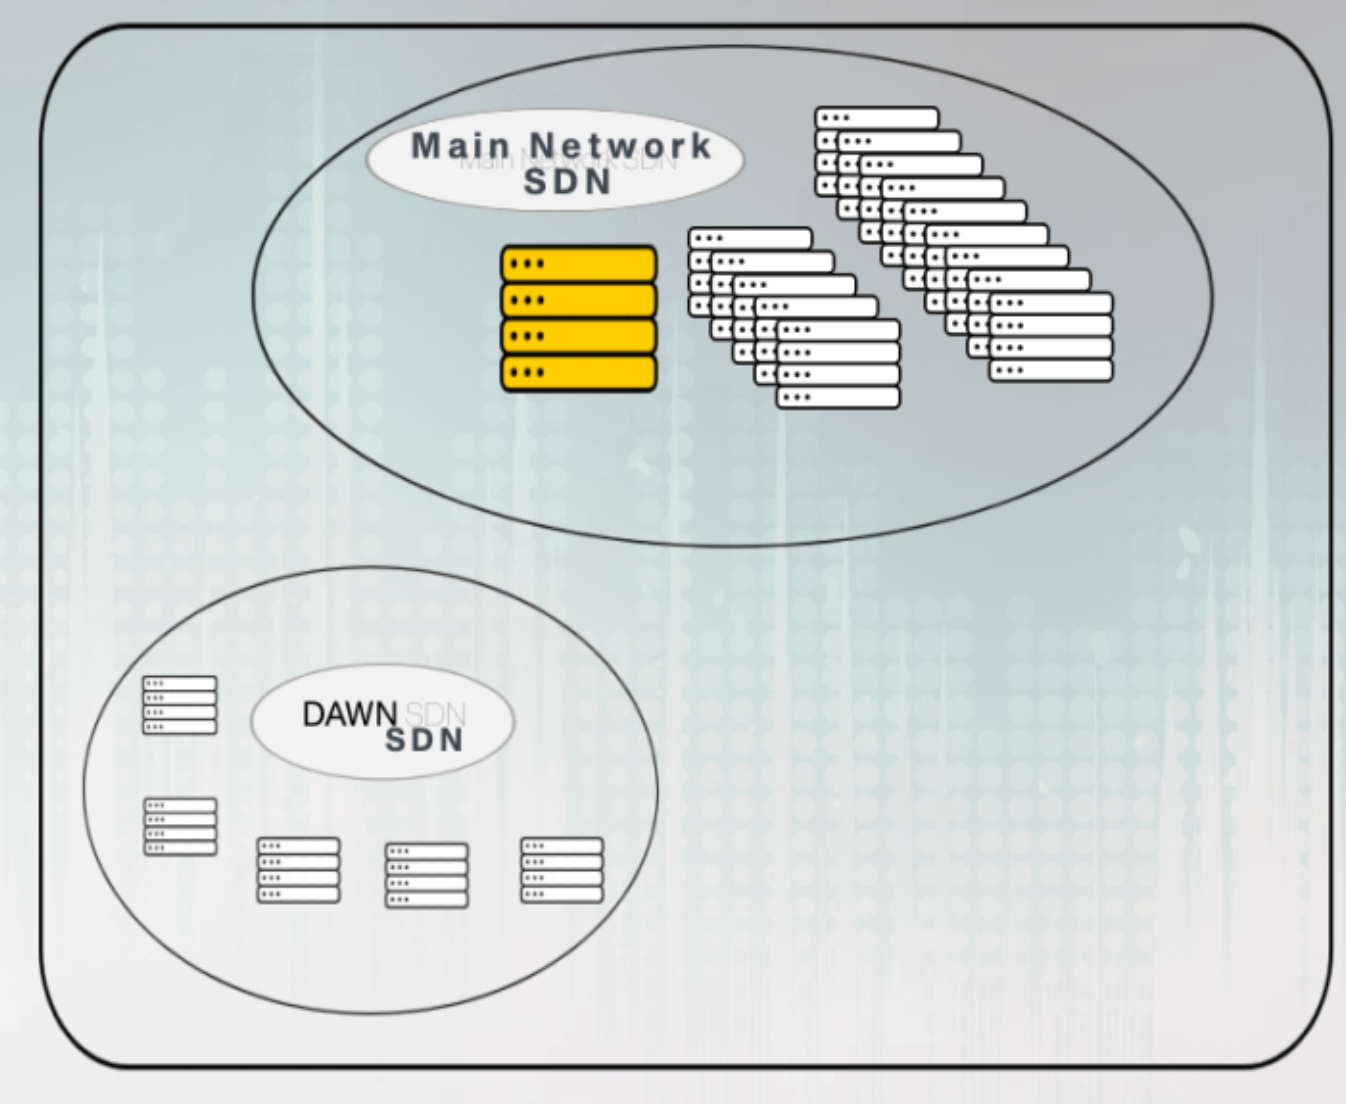
\includegraphics[scale=0.32]{fig1.png}
\caption{DAWN Auxiliary SDN}
\end{figure}

Role of SDN in DAWN
With its flexible, dynamic, and programmable nature, Software Defined Networks (SDN) can offer advancements in functionality previously unavailable with traditional network infrastructure due to its improved performance, scalability, and management [19].
The architecture of SDN contains three core planes: the control, data, and application planes. Housed within the SDN controller, the control plane is the strategic decision-making epicenter of the network, overseeing devices that forward packets in the data plane [19]. It handles the dispatch devices that forward packets on the data plane [19]. In a standard network setup, these transmissions are based on factors like congestion, service priority, and a link's status [19]. The data plane is the physical worker, containing devices like switches and routers, which are programmed and overseen by the control plane. They operate under the directive of the rules established by the controller[19]. 

Furthermore, the application plane communicates with the devices on the network infrastructure through the SDN controller. This plane contains applications that can request network services from the controller, notably load balancers and firewalls [19]. To achieve this, applications interact with the controller through a Northbound interface; conversely,  the data plane communicates with the control plane using a Southbound interface like Openflow protocol [19]. OpenFlow centralizes control logic dynamically, managing flow tables in real time,  thus ensuring flexibility in a rapidly evolving network [19]. 

In the context of DAWN's auxiliary SDN, the control plane shoulders the responsibility of activating preprocessors and steering data plane instructions to reroute traffic accordingly. This DAWN control plane establishes communication links with the principal SDN's control plane, ensuring cohesive network operations. During threats, the DAWN SDN triggers the DAWN data plane to redirect traffic to preprocessors. This channeling will help in isolating the main SDN from the incoming attack.

Regarding the DAWN application plane, it undertakes the crucial tasks of alerting administrators of attack status, bridging a communication interface between the DAWN and main SDN, and delving into advanced operations like deep packet inspections and machine learning. Any software tool or service provided during an attack and utilizing network data could be hosted here. The server preprocessors in DAWN can be considered a combination of the data and application plane, and this is made feasible with the help of Network Function Virtualization (NFV). 

Role of NFV in DAWN
Network Function Virtualization (NFV) has revolutionized traditional network operations by decoupling network functions from proprietary hardware. These virtualized functions now run as software instances on switches, routers, and high-volume storage [7]. 

The NFV architecture is a complex system that comprises three main components: the NFV Infrastructure (NFVI), Virtual Network Functions (VNFs), and the Management and Orchestration (MANO) [15]. The NFVI offers physical resources and a virtualization layer [15]. It utilizes cost-effective x86 computing hardware, software, hypervisors, and virtual machines. The NFVI provides physical resources for processing, data storage, and network connection for NFVs under its management [15]. By placing the virtualization layer on top of the hardware, the NFVI allows logical resource partitioning for NFV deployment, enabling the creation of complex networks without geographic limitations [15]. 
The NFVs, conversely, are virtualized applications that execute specific network functions such as routing, switching, SD-WAN, and firewalls [15]. They can be deployed swiftly and minimize the need for onsite setup expertise, and can have agility and adaptability [15]. Finally, there is the NFV MANO layer, which oversees the lifecycle of VNFs and orchestrates resources across the NFVI. Each of these components plays a critical role in ensuring the success of the NFV architecture.
[15].

NFV's unmatched flexibility and scalability allow networks to respond dynamically to various demands without necessitating extensive hardware replacements. NFV also improves the role of hardware servers, dynamically managing load distribution and simulating multiple virtual servers on a single platform [7]. 

The transformative potential of NFV is fully realized within DAWN, particularly in countering dynamic threats like DDoS attacks. DAWN leverages NFV's flexibility to seamlessly adapt, utilizing its dynamic provisioning of resources, virtual functions, and network modification. NFVs augment servers' capabilities, and DAWN capitalizes on that to enhance its preprocessor hardware servers, ensuring the ability to simulate virtual preprocessors and load management [7]. NFVs allow DAWN access to various defense tools to address specific threats enabling the installation of robust defense mechanisms. 

Bouras et al. highlight the complementary nature of SDN and NFV: "Although SDN and NFV are two extremely different technological suggestions, their combination offers benefits in favor of succeeding high network efficiency and performance." [7]. This collaboration ensures an adaptive defense mechanism, promising unwavering security against evolving threats.
Installing NFVs in Dawn will be at the application layer within the preprocessors for traffic analysis, intrusion detection, processing blacklist and whitelists, machine learning, and other high decision-making processes. NFVs will also be installed at the data plane within the preprocessors and handle traffic directions based on predefined rules and in connection with the DAWN SDN's order. The control plane will also have a version of NFV to facilitate dynamic real-time decision-making. Plus NFVs can help update the whitelists and blacklists, ensuring they are up to date and quickly being disseminated to the preprocessors.

\section{TYPES OF DDoS ATTACKS}

DDoS resource depletion attacks, a subset of DoS attacks, aim to exhaust resources in the victim's network [18]. These attacks frequently employ botnets, extensive networks of compromised devices [18]. Often, these compromised devices belong to unsuspecting individuals whose devices have been infected by malware. Controlled by a bot master, these bots are commanded to flood target systems with an overwhelming number of requests [18]. In traditional networks, distinguishing between legitimate and bot-generated requests is challenging, as while networks can authenticate the user, they often cannot authenticate the traffic [18].

Volumetric Attacks
Volumetric attacks, also known as flooding attacks, are the most prevalent types of DDoS attacks. Their primary objective is to inundate a network's infrastructure by flooding it with excessive internet traffic, thereby saturating the victim's bandwidth [1]. Specific forms of volumetric attacks include:
In UDP Floods, attackers send a multitude of User Datagram Protocol (UDP) packets to random ports on the target system, overwhelming its capacity [21].
In DNS Amplification, this strategy, botnets send numerous requests to DNS servers, spoofing the return address to make it appear as though the victim's system is the requester. This results in an overwhelming response directed at the victim.
In ICMP Ping Flood, attackers bombard the victim with a series of ICMP Echo Requests, causing the system to be swamped by the resulting traffic [21].

Protocol Attacks: 
Protocol attacks exploit vulnerabilities within the Layer 3 and Layer 4 of the protocol stack. Their primary aim is to target the processing capabilities of the victim's server by leveraging weaknesses in the network layer [1]. A notable instance of a protocol attack is the SYN Flood. In this attack, a bot sends a SYN request to a target server and spoofs its IP address. As a result, the victim server is unable to locate the spoofed IP for the second part of the handshake (SYN-ACK), leading to resource consumption and rendering the server unresponsive to legitimate traffic [21].

Application Layer Attacks:
 Application layer attacks, which are subtle and often difficult to detect, target specific points on servers where web pages are generated and served in response to HTTP requests. During these attacks, web servers or applications are manipulated into responding to what appear to be legitimate requests [1]. A prime example of such an attack is the HTTP flood, wherein the attacker disseminates an excessive number of HTTP requests, overwhelming web servers and forcing them to produce a significant volume of responses.

Low and Slow Attacks: 
Low and slow attacks involve sending limited and deliberately slow traffic to target a server's resources, making the traffic difficult to differentiate from regular user activity. Their main objective is to delay or deny services to genuine users [20]. These attacks can persist for prolonged periods and may be orchestrated by a single computer utilizing tools like Slowloris and R.U.D.Y [20]. Essentially, low and slow attacks intend to tie up all server threads with these gradual requests, thus hindering genuine users from accessing the intended service [20]. To achieve this, attackers employ various techniques including sending partial HTTP headers, dispatching slow HTTP POST requests, or using TCP traffic. For example, Slowloris transmits sluggish partial HTTP headers, R.U.D.Y. generates slow HTTP POST requests, while the Sockstress attack leverages vulnerabilities in the TCP/IP handshake [20].

\section{LOAD BALANCING IN DAWN}

Why Load Balancing is Crucial in DDoS Mitigation
Load balancing is an essential solution to the challenges posed by DDoS attacks, ensuring efficient resource utilization [18]. The ability to distribute incoming traffic uniformly across multiple servers ensures that no server is overwhelmed. This distribution maximizes available resources, securing continuous service availability and preventing servers from overloading [18]. This approach simplifies the system's response time, avoiding potential bottlenecks from hampering performance. 

DAWN's Approach to Load Balancing: 
A dynamic hardware preprocessor activation mechanism is at the core of DAWN's strategy. When the DAWN SDN captures traffic, it smartly redistributes this traffic based on the computational capacity of each server preprocessor. Load balancing in DAWN can be approached in two ways. One focuses on speed, activating a new preprocessor even if the existing ones aren't fully utilized. The other, which is our preferred method, emphasizes efficiency. This choice is rooted in its commitment to optimal resource utilization.
Thanks to the integration of DAWN SDN and NFVs, DAWN boasts collaborative and redundant capabilities, both of which are pivotal to its strategy. DAWN SDNs are equipped to communicate and distribute excessive loads among their preprocessors or partnering DAWN SDNs. Such cooperation fosters a setting where they can collaboratively identify and counteract malicious traffic in real time, bolstering the system's defense against DDoS attacks.

Theoretical Assessment of DAWN's Load-Balancing Capability:
Our theoretical exploration suggests that simulating DAWN's load-balancing capability is foundational in assessing its potential. It's important to note that the efficiency of any load-balancing approach can vary based on the specific configuration of the balancer in play. Some balancers, tailored for high-traffic scenarios, may dynamically adapt to changing traffic demands. In contrast, others might show limited adaptability. We've set up initial simulation (https://github.com/allali7/DAWN-SDN), offering a basic glimpse into DAWN's load distribution framework. While these simulations provide an elementary view, they pave the way for more sophisticated testing and refinements in the future.

Load Balancing Explanation:
Central to our load-balancing approach is the judicious allocation of packets to the preprocessors. Upon the arrival of a new packet, the system undergoes a sequence of checks, as seen in Fig 2.


\begin{figure}[h]
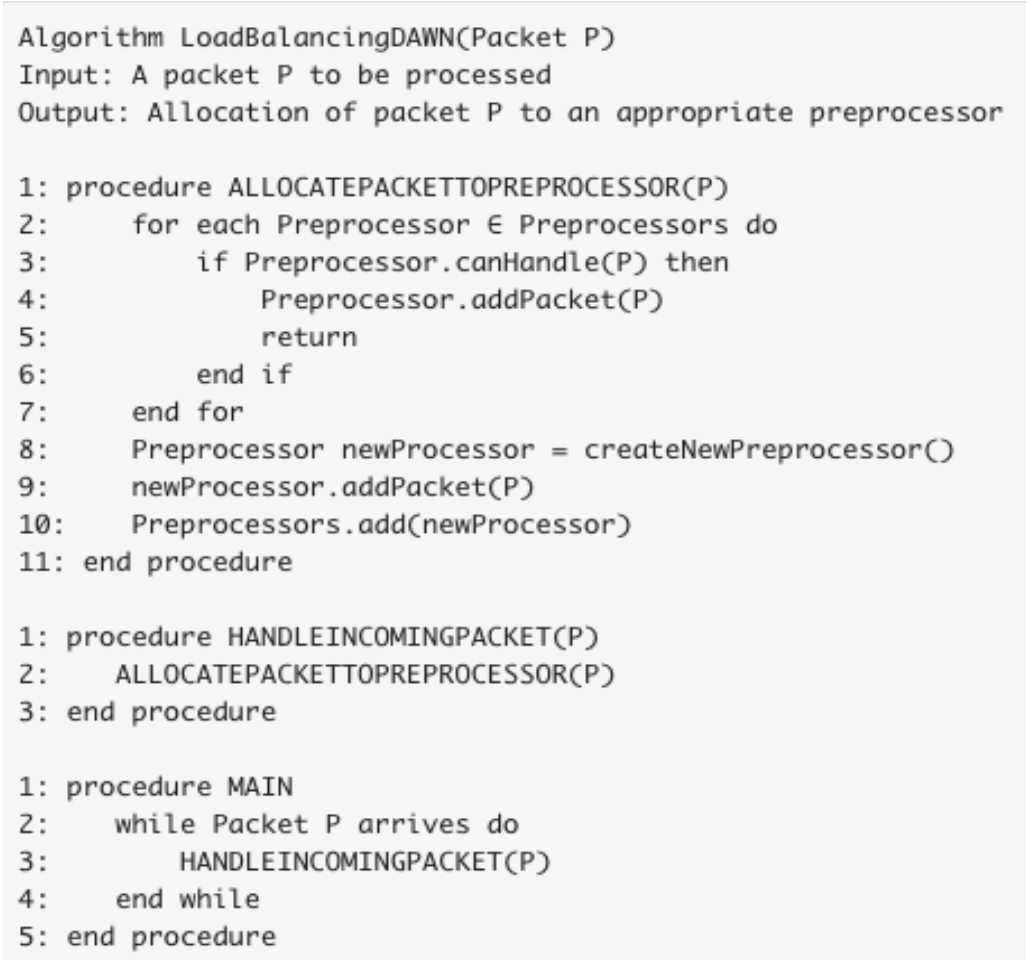
\includegraphics[scale=0.46]{fig2.png}
\caption{Load Balancing Algorithm in DAWN }
\end{figure}


1. Initially, it determines if there exists a virtual preprocessor with the requisite capacity for the packet. If a suitable one is identified, the packet is channeled to this preprocessor.
  
2. Failing that, the system then seeks out a physical preprocessor with sufficient capacity. Should one be found, the packet is directed to this unit.
  
3. In cases where neither virtual nor physical preprocessors can take on the packet, the system responds by instantiating a new physical preprocessor and then assigning the packet to it.
The underlying objective of this methodology is to optimize the utility of both virtual and physical preprocessors. By doing so, it aims to prevent undue stress on any single unit, while also initiating the creation of new preprocessors only as a last resort. This approach not only ensures a balanced distribution of processing tasks but also mitigates the risk of any particular preprocessor emerging as a processing choke point. Thus, the design guarantees that packets navigate the system with maximum efficiency, respecting the individual capacity limits of each preprocessor. Furthermore, in the event of potential SDN failures, DAWN aims to maintain its robustness by falling back on its preprocessors' NFV inherent load-balancing abilities, ensuring continuous operation. 

\section{DETECTION ON MAIN NETWORK SDN}
Detection of attacks in the main network SDN involves mechanisms implemented with-in the main SDN, leveraging its network-wide visibility to enhance attack detection accuracy. One such mechanism is Time-Cap Alerts, which trigger actions upon identifying attacks or unusual surges that surpass predefined time limits. These alerts can detect anomalies like login attempts from unfamiliar locations. A proposed framework utilizes SDN architecture to optimize real-time network flow management, ensuring the end-to-end timing requirements met. Machine Learning is applied to DDoS detection, analyzing network traffic and user behavior to identify patterns indicative of attacks, such as sudden spikes in traffic. A study explores ML techniques like Random Forest (RF) and Decision Tree (DT), achieving high accuracy in DDoS attack packet detection [6][9]. The code snippets illustrating the use of these algorithms.

%%%%TWO SOURCES HERE

\lstset{basicstyle=\small, basewidth=0.5em}
\begin{minipage}{0.8\linewidth}
\begin{lstlisting}[language=Python, caption=Decision Tree and Random Forest Classifiers [sourCE]]
# Decision Tree Classifier
dt = DecisionTreeClassifier()
dt.fit(X_train, y_train)
y_pred = dt.predict(X_test)

# Random Forest Classifier
rf = RandomForestClassifier(
    n_estimators=100)
rf.fit(X_train, y_train)
y_pred = rf.predict(X_test)
\end{lstlisting}
\end{minipage}
\begin{figure}[h]
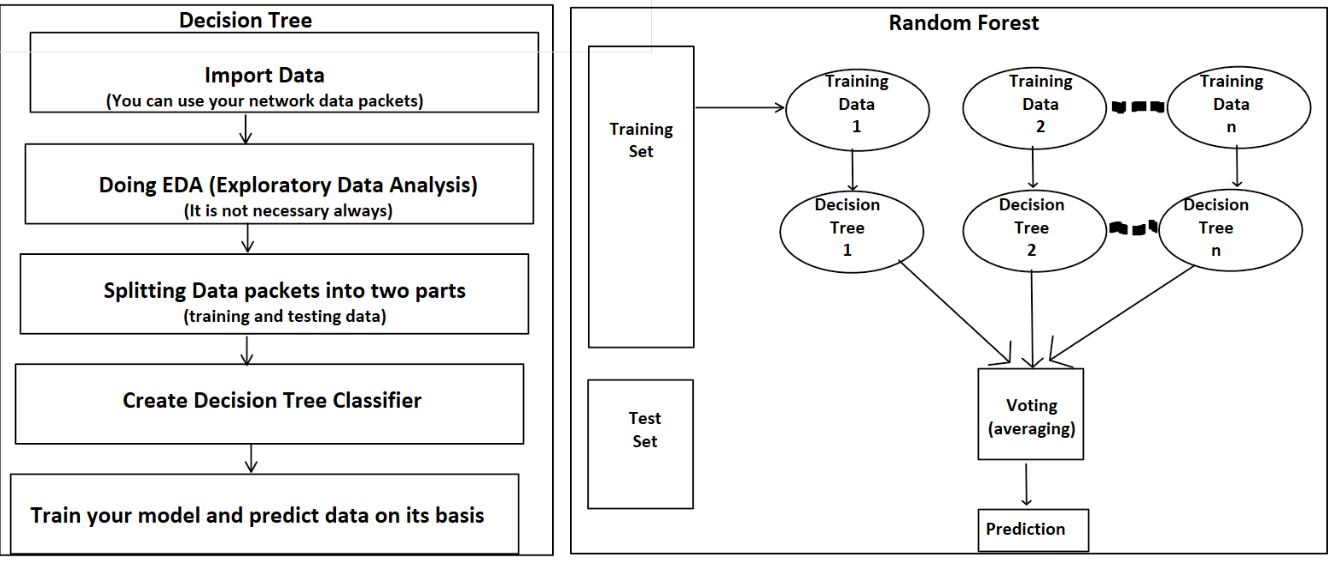
\includegraphics[scale=0.36]{fig3.png}
\caption{Decision Tree Classifier and Random Forest Classifier [source]}
\end{figure}

The paper highlights the advantages and disadvantages of DT and RF. Deep packet inspection enhances detection by analyzing packet data, employing techniques like anomaly detection, traffic profiling, entropy-based analysis, rate-based detection, traffic correlation, and signature-based and flow-based approaches. "Low and Slow DDoS attack" detection involves sophisticated techniques including connection count monitoring, behavior clustering, and heuristic thresholds. Unusual access patterns are monitored to detect potential compromises. The provided source code demonstrates a function to detect DDoS attacks based on abnormal traffic volume and rate, utilizing simulated functions to retrieve packet counts and send alerts [12].

\lstset{basicstyle=\small, basewidth=0.5em}

\begin{minipage}{0.75\linewidth}
\begin{lstlisting}[language=Python, caption=DDoS Detection Function]
# Define function to detect DDoS attacks
def detect_ddos_attack(traffic_data):
    threshold_volume = 1000
    threshold_rate = 5
    
# Check for DDoS attacks based on traffic volume and rate
    if (current_packets > threshold_volume or 
        packets_per_second > threshold_rate):
        msg = "DDoS detected! Unusual access pattern."
        send_alert(msg)

# Function to simulate retrieving current packet count
def get_current_packets():
    import random
    return random.randint(500, 2000)
\end{lstlisting}
\end{minipage}

By employing advanced algorithms and updating detection models, DAWN SDN controllers enhance DDoS attack detection, ensuring timely and effective responses for network mitigation.

\section{MACHINE LEARNING IN DAWN}
Using Machine Learning (ML) in Software-Defined Networks (SDN) for DDoS detection. It highlights potential ML algorithms like Isolation Forest, One-Class Support Vector Machines, and Auto encoders. The use of various neural network models for detecting slow and low malicious traffic is mentioned. The researchers have been identified such as Decision Tree and Random Forest algorithms achieved the highest accuracy, with Decision Tree being favored due to its lower computation time [22]. ML techniques are applied for traffic classification, leading to the deployment of security rules against DDoS attacks in SDN. In the context of 5G networks, a deep Kalman back propagation neural network is used for DDoS detection, achieving a 97.49\% detection rate [22]. Another approach involves using a split-machine learning system and network slicing to identify DDoS attacks in 5G and beyond networks. ML’s role in identifying attack patterns includes anomaly detection, real-time analysis, automated response triggering, attack classification, adaptive defense, and behavioral analysis. The process involves data collection, feature extraction, labeling, training, validation, and deployment of ML models [22]. The significance of updating and training ML models is emphasized, enabling adaptability to new attacks, handling zero-day attacks, reducing false positives/negatives, learning from legitimate traffic, mitigating model drift, and improving defense strategies for long-term network performance, rapid threat response, risk mitigation, and continuous improvements [22].

\section{DEFENSE OF ATTACK IN DAWN}
A.DAWN SDN Defense:

i. Activation:
The DAWN SDN rises into action upon receiving a notification from the main network SDN indicating potential threats or ongoing attacks.

ii. Traffic Management:
Whitelisting: Ensures that traffic emanating from previously verified and trusted sources receives priority, minimizing disruptions to genuine users [1].
Blacklisting: By maintaining a record of known malicious entities, DAWN SDN can deny them access, thereby reducing potential threats.

iii. Signature List Distribution:
DAWN SDN circulates profiles of known harmful packet structures to preprocessors, providing them with the knowledge required to instantly identify and counteract specific threats.

iv. Traffic Control:
Rate Limiting: By modulating the traffic influx, DAWN SDN safeguards network resources from being overwhelmed, particularly during Distributed Denial-of-Service (DDoS) attacks. There is research by Patil et al. on how to dynamically rate limit based based on packet history
IP Filtering: This acts as an initial barrier, curtailing potentially hazardous traffic originating from previously identified malicious IPs or IP clusters [1][23].

v. Virtual Defense Mechanisms:
Firewall: Acts as a virtual gatekeeper, DAWN SDN's firewall restricts entry to dubious traffic, leveraging predefined rules and dynamic assessments [1].
Deep Packet Inspection (DPI): Beyond just header information, DPI delves deep into the packet's content, scouting for malicious payloads or patterns [1].

vi. Anomaly Detection:
DAWN SDN constantly observes the fluctuations and patterns of network traffic, sounding alarms when it detects inconsistencies or unusual patterns, and rerouting such traffic for closer inspection. Advanced machine learning techniques like the Traffic-Intrusion Detection System (T-IDS) can be used here [1].

vii. Communication with Main SDN:
To stay one step ahead of evolving threats, DAWN SDN periodically relays frontline threat data to the primary SDN, ensuring network-wide vigilance. 

B. DAWN Preprocessor Defense:

i. Activation:
The preprocessors, specialized defense units, become fully operational when signaled by the DAWN SDN, mainly during high-risk situations.

ii. Signature-based Detection:
Preprocessors meticulously scan each packet against a database of malicious signatures, ensuring known threats are identified and neutralized immediately [1].

iii. Anomaly Detection:
Going beyond signatures, preprocessors also look for abnormal traffic behavior, which might indicate novel or evolving threats.

iv. Protocol Verification:
By analyzing protocol adherence, preprocessors can detect nefarious activities like SYN flood attacks, which exploit handshake protocols or packets that deviate from standard size and flag configurations.

v. Hardware-Level Defense:
Firewall: Preprocessors' hardware-based firewalls offer an additional, robust layer of defense, rapidly filtering out flagged content.
DPI: At this level, DPI operates with enhanced granularity, investigating the minutiae of packet content, ensuring nothing slips through [1].

vi. Behavioral Analysis:
By tracking parameters such as traffic volume, frequency, and communication patterns, preprocessors can discern potentially malicious intent even if the threat doesn't match any known signature.

vii. Feedback Loop to DAWN SDN:
Preprocessors constantly update DAWN SDN with fresh intelligence, recommending additions or modifications to blacklists, whitelists, or signature databases.

Through a collaborative approach, DAWN SDN and DAWN preprocessors together create a multi-layered defense fortress. This coordinated strategy ensures optimal network protection, with each component playing a pivotal role in countering cyber threats [1].

\section{COMPARISON WITH EXISTING SOLUTIONS}
A. Overview of Cisco Guard, Akamai’s Kona site defender, and Cisco secure DDoS edge

Cisco Guard:
Cisco Guard is a DDoS attack mitigation tool designed to safeguard network traffic. Deployed at the backbone level, it activates upon detecting potential threats, diverting suspicious traffic away from its targeted zone for analysis. This system is adept at learning from consistent traffic behaviors, which assists in distinguishing between legitimate and malicious traffic. Anti-spoofing techniques handle deceptive traffic, while statistical methods tackle straightforward threats. Cisco Guard's flexibility allows it to offer protection across varied scales – from singular servers to expansive ISPs – and its feedback mechanisms help it adjust rapidly to evolving attack strategies [8].

Akamai’s Kona site defender:
Operating as a top-tier cloud-based web application firewall (WAF), Kona Site Defender primarily protects web applications and their associated APIs, emphasizing thwarting DoS attacks. Anchored in the Akamai Intelligent Edge Platform, it relies on an extensive reverse proxy infrastructure for traffic management. This setup allows it to promptly address network-layer DoS threats at its periphery while managing more intricate application-layer attacks, preserving a smooth experience for genuine users. The WAF regularly receives updates from Akamai Threat Research, ensuring its defenses remain up-to-date. With specialized features like advanced API security and CI/CD integration, Kona also provides real-time notifications, granular attack insights, and is optimized for streamlined SIEM integration [14].


Cisco secure DDoS edge:
Tailored to combat DDoS threats targeting the 5G network edge, Cisco Secure DDoS Edge Protection is particularly vigilant against malicious IoT devices and user equipment. With its operations centered around 5G ecosystems, it scrutinizes GPRS Tunneling Protocol (GTP) traffic to thwart malevolent entities before they penetrate deeper layers of the network. This system's strategic positioning close to potential threat origins ensures timely threat detection and mitigation. Its integration within a docker container in IOS XR, paired with a centralized controller, means it functions without the need for external connectivity. Designed to tackle a spectrum of threats, from IoT-based attacks to GTP tunnel breaches, its streamlined processing – exemplified by its localized handling of NetFlow data on routers – boosts its detection and mitigation speeds [13].



B. Comparison of their DDoS mitigation strategies with DAWN
\begin{table}[h]
    \centering
    \small
    \begin{tabular}{|p{1.6cm}|p{1.2cm}|p{1.2cm}|p{1.2cm}|p{1.2cm}|}
        \hline
        & \textbf{Cisco Guard} & \textbf{Akamai Kona} & \textbf{Cisco secure DDoS Edge} & \textbf{DAWN} \\
        \hline
        \textbf{Traffic} \newline \textbf{Diversion} & Diverts suspicious traffic. & Rejects at edge; absorbs application-layer. & 5G edge prevention. & Combines diversion with behavioral analytics. \\
        \hline
        \textbf{Learning} \newline \textbf{Capabilities} & Learns traffic behaviors. & Uses Akamai Research updates. & - & Machine learning with real-time insights. \\
        \hline
        \textbf{Attack} \newline \textbf{Handling} & Anti-spoofing and statistics. & Targets app-layer/API threats. & Handles IoT/DNS attacks. & Real-time, signature-based detections. \\
        \hline
        \textbf{Protection} \newline \textbf{Levels} & From analysis to strong. & IP controls, app-layer DoS protection. & 5G edge focus. & AI-driven, threat sandboxing. \\
        \hline
        \textbf{Scalability/} \newline \textbf{Adaptability} & Manages zones. & Scales with global platform. & Ready for 5G traffic. & Dynamic auto-scaling, optimized processing. \\
        \hline
    \end{tabular}
    \caption{Comparison of DDoS mitigation strategies.}
    \label{tab:comparison}
\end{table}

C. Comparative Analysis: Performance, Efficiency, Scalability, and Adaptability

Performance:
Cisco Guard stands out in its dynamic response to varying attack patterns, leveraging its closed-loop feedback mechanism to handle spoofed and non-spoofed traffic efficiently [8]. With its cloud infrastructure and wide-reaching global distribution, Akamai's Kona Site Defender promptly counters network and application-layer DoS threats [14]. Meanwhile, the strength of Cisco Secure DDoS Edge lies in its proximity to potential threats, ensuring swift detection and mitigation, further bolstered by direct NetFlow data processing on routers [13]. DAWN differentiates itself by adopting a hybrid traffic diversion strategy and advanced behavioral analytics, ensuring a robust defense mechanism even under heightened attack scenarios. Furthermore, DAWN demonstrates a heightened proficiency in addressing 5G-specific threats, an area where Kona and Guard might be less specialized.

Efficiency:
Cisco Guard's continuous adaptation to standard traffic patterns over time fortifies its DDoS mitigation efficiency [8]. On the other hand, Akamai's Kona Site Defender is equipped with a frequently updated firewall, backed by Akamai Threat Research, and boasts robust API security features, ensuring a holistic defense against threats [14]. Cisco Secure DDoS Edge streamlines its efficiency by prioritizing GTP traffic, thereby directly targeting principal avenues of potential 5G attacks [13]. DAWN's approach is a blend of real-time traffic analysis and signature-based detection, allowing it to discern between benign and malicious requests quickly.

Scalability:
Cisco Guard's scalability is evident in its capability to oversee multiple zones, albeit within its predefined limits [8]. Contrastingly, Akamai's Kona Site Defender enjoys the backing of a globally distributed platform, enabling it to gracefully scale as traffic demands fluctuate [14]. Cisco Secure DDoS Edge is inherently prepared for the substantial traffic influx that 5G is anticipated to usher in [13]. DAWN, utilizing cloud-native paradigms, excels in dynamic resource provisioning. Moreover, its auto-scaling features ensure resilience against sudden and unexpected traffic spikes.

Adaptability:
Adapting to the changing dynamics of web traffic is one of Cisco Guard's hallmarks, enabling it to tailor its defenses according to evolving traffic patterns [8]. Akamai's Kona Site Defender is ever-evolving, staying abreast of the latest web threats thanks to its continual research-driven updates [14]. Cisco Secure DDoS Edge showcases its flexibility and adaptability through docker container integration within IOS XR and centralized controller architecture [13]. DAWN distinguishes itself by leveraging real-time machine learning algorithms and SDN capabilities, dynamically adjusting its defenses to known and emergent cyber threats, and ensuring a proactive and responsive security posture in an ever-shifting digital landscape. 

\section{Integration and Standalone Deployment of DAWN}
A. DAWN as an Integrative Solution: 
One of DAWN's predicted significant advantages is its compatibility with existing security infrastructures. Organizations can layer DAWN onto their current DDoS mitigation solutions, enhancing their defenses with DAWN's advanced machine learning, behavioral analytics, and 5G-specific threat detection algorithm. This integrative capability ensures businesses can harness DAWN's cutting-edge features without completely overhauling their established security measures. DAWN can address gaps in other solutions by acting as a complementary layer, particularly in rapidly evolving areas like 5G security.

B. DAWN as a Standalone Protector: 
On the other hand, for businesses looking for a comprehensive, modern solution or those setting up new infrastructures, DAWN could serve as a robust standalone defender. Its emphasis on traffic analysis, real-time examination, and adaptability makes it a formidable shield against various DDoS attacks. Moreover, its focus on the core network's edge positions it as a guardian for high-risk servers that require consistent uptime. DAWN should scale dynamically, making it suitable for businesses of varying sizes and traffic demands.

Whether DAWN is incorporated as an added layer or employed as the primary line of defense, it has the potential to provide a coherent system designed for the challenges of modern networked environments.

\section{Challenges and Future Directions}
A. Challenges in Implementing DAWN
Technological Challenges:
The very nature of a Distributed Adaptive Workflow Network like DAWN demands the integration of diverse technologies and systems. Achieving a seamless operation amidst this diversity can be a complex undertaking. Potential issues could emerge in the form of compatibility conflicts among the different systems. Much testing is needed is this area. 

Operational Challenges: 
Managing DAWN operationally implies a need for intricate coordination across multiple teams and departments. This mandates clear and efficient communication to ensure everyone aligns with the overarching objectives. Operational complexities could also arise from challenges related to data management and in-depth analysis. Much testing needs to be done in the future. 

Security Challenges: 
Given the increasing cyber threats, fortifying the security parameters of DAWN is paramount. While measures like firewalls, intrusion detection systems, and encryption lay the foundational security, challenges might arise in maintaining encrypted communication channels and implementing nuanced access control. Extensive testing needs to be done in this area.

Economic Considerations: 
Initial costs tied to DAWN's implementation might be steep, though the potential long-term benefits could justify the upfront investment. Moreover, as technology advances and becomes more accessible, the costs associated with such high-end systems are likely to diminish over time.

While it is expected that the cost of a small individual DAWN server setup, along with NFV and SDN components, would likely exhibit cost-efficiency compared to other prevailing solutions, providing a precise numerical estimate is beyond the scope of this paper. Due to the highly tailored nature of these tools, pricing details are not openly available, and acquiring a quote necessitates specific customization. While we have explored these options, as of now, the exact figures remain undisclosed.

B. Future Directions for DAWN
Technological Enhancements:
Future iterations of DAWN can benefit from advancements such as novel summation patterns, system material properties optimization, skill-mounted generators, and refined wireless power transfer techniques.
Agile Workflow Management: 
Implementing an Agile methodology can foster transparency and flexibility, ensuring DAWN remains adaptable to changing requirements

C. Other attacks and DAWN: 
Protection against 5G-specific attacks: 
As 5G architectures are uniquely tailored to offer low latency with expansive connectivity, they become vulnerable to specific attacks. DAWN is designed to shield against threats like Volumetric DDoS attacks, SYN Flood, UDP Flood, and HTTP flood attacks. Its inherent features, such as NFV-based preprocessors and machine learning modules, can screen and process traffic in real-time, thwarting malicious intents.

Addressing Signaling Storms in 5G: 
The evolution of 3GPP mobile broadband networks has led to challenges like signaling storms, exacerbated by increased smartphone usage and data-intensive social applications. DAWN could potentially offer solutions through network architecture optimization and enhancing control signaling efficiency.

In summary, while DAWN holds immense promise as a revolutionary tool against cyber threats, its successful implementation and evolution demand rigorous planning, testing, and continuous adjustments. The future seems promising for DAWN, especially as it sets its sights on addressing the nuanced challenges presented by the proliferation of 5G networks.

\begin{thebibliography}{00}
\bibitem{b1}
A. Lohachab and B. Karambir, "Critical Analysis of DDoS—An Emerging Security Threat over IoT Networks," in Journal of Communications and Information Networks, vol. 3, no. 3, pp. 57-78, Sept. 2018, doi: 10.1007/s41650-018-0022-5.

\bibitem{b2} Agency, N. D. (n.d.). Kona ddos defender - web performance, Cloud Security \& Cloud Computing Services. Arturai. \url{https://www.arturai.com/en/all-products/kona-ddos-defender}

\bibitem{b3} Abrams, L. (2021, September 20). VoIP.ms phone services disrupted by ddos extortion attack. BleepingComputer. \url{https://www.bleepingcomputer.com/news/security/voipms-phone-services-disrupted-by-ddos-extortion-attack/}

\bibitem{b4} A. S. Mamolar, Z. Pervez, Q. Wang and J. M. Alcaraz-Calero, "Towards the Detection of Mobile DDoS Attacks in 5G Multi-Tenant Networks," 2019 European Conference on Networks and Communications (EuCNC), Valencia, Spain, 2019, pp. 273-277, doi: 10.1109/EuCNC.2019.8801975.

\bibitem{b5} Ax Sharma - Sep 22, 2021 1:03 pm UTC. (2021, September 22). Phone calls disrupted by ongoing ddos cyber attack on voip.ms. Ars Technica. \url{https://arstechnica.com/gadgets/2021/09/canadian-voip-provider-hit-by-ddos-attack-phone-calls-disrupted/}

\bibitem{b6} Bhamidipaty, A. (2021, November 15). IBM developer. \url{https://developer.ibm.com/learningpaths/get-started-anomaly-detection-api/what-is-anomaly-detection/}

\bibitem{b7} C. Bouras, A. Kollia and A. Papazois, "SDN \& NFV in 5G: Advancements and challenges," 2017 20th Conference on Innovations in Clouds, Internet and Networks (ICIN), Paris, France, 2017, pp. 107-111, doi: 10.1109/ICIN.2017.7899398.

\bibitem{b8} Cisco Guard Configuration Guide (Software Version 6.0) - product overview [Cisco Guard ddos mitigation appliances]. Cisco. (2007, November 2). https://www.cisco.com/en/US/docs/security/anomaly\_detection
\_mitigation/appliances/guard/v6.0/configuration/guide/Intro.html}

\bibitem{b9} F. Zhou, W. Huang, Y. Zhao, Y. Shi, X. Liang and X. Fan, "ENTVis: A Visual Analytic Tool for Entropy-Based Network Traffic Anomaly Detection," in IEEE Computer Graphics and Applications, vol. 35, no. 6, pp. 42-50, Nov.-Dec. 2015, doi: 10.1109/MCG.2015.97.

\bibitem{b10} Hossain, M. (1633, March 26). OpenFlow SDN Controller-how 5G will leverage the concept of it?. LinkedIn. \url{https://www.linkedin.com/pulse/openflow-sdn-controller-how-5g-leverage-concept-monowar-hossain/}

\bibitem{b11} J. Gojic and D. Radakovic, "Proposal of security architecture in 5G mobile network with DDoS attack detection," 2022 7th International Conference on Smart and Sustainable Technologies (SpliTech), Split / Bol, Croatia, 2022, pp. 1-5, doi: 10.23919/SpliTech55088.2022.9854338.

\bibitem{b12} J. Roldán-Gómez, J. Boubeta-Puig, J. M. Castelo Gómez, J. Carrillo-Mondéjar and J. L. Martínez Martínez, "Attack Pattern Recognition in the Internet of Things using Complex Event Processing and Machine Learning," 2021 IEEE International Conference on Systems, Man, and Cybernetics (SMC), Melbourne, Australia, 2021, pp. 1919-1926, doi: 10.1109/SMC52423.2021.9658711.

\bibitem{b13} Kandula, R. (2022, August 5). Stop ddos at the 5G network edge. Cisco Blogs. \url{https://blogs.cisco.com/sp/stop-ddos-at-the-5g-network-edge}

\bibitem{b14} Kona Site Defender, Product Brief, Akamai (n.d.-a) \url{https://www.akamai.com/site/en/documents/product-brief/akamai-kona-site-defender-product-brief.pdf}

\bibitem{b15} Leonhardt, A. (2023, August 2). Defining the elements of NFV Architectures. Interconnections - The Equinix Blog. \url{https://blog.equinix.com/blog/2019/10/17/networking-for-nerds-defining-the-elements-of-nfv-architectures/}

\bibitem{b16} L. Hardesty, "Cybersecurity: Congress Grills TikTok; 5G Propels DDoS Attacks," FierceWireless, 23 July 2023. [Online]. Available: \url{https://www.fiercewireless.com/5g/cybersecurity-congress-grills-tiktok-5g-propels-ddos-attacks}.

\bibitem{b17} M. Lefoane, I. Ghafir, S. Kabir and I. -U. Awan, "Unsupervised Learning for Feature Selection: A Proposed Solution for Botnet Detection in 5G Networks," in IEEE Transactions on Industrial Informatics, vol. 19, no. 1, pp. 921-929, Jan. 2023, doi: 10.1109/TII.2022.3192044.

\bibitem{b18} N. Gokul and S. Sankaran, "Modeling and Defending against Resource Depletion Attacks in 5G Networks," 2021 IEEE 18th India Council International Conference (INDICON), Guwahati, India, 2021, pp. 1-7, doi: 10.1109/INDICON52576.2021.9691522.

\bibitem{b19} Polat, H., Polat, O., \& Cetin, A. (2020a, February 1). Detecting ddos attacks in software-defined networks through feature selection methods and Machine Learning Models. MDPI. \url{https://www.mdpi.com/2071-1050/12/3/1035}

\bibitem{b20} What is a low and slow attack? - cloudflare. (n.d.).\url{https://www.cloudflare.com/learning/ddos/dd}

\bibitem{b21}A. Girma, M. Garuba, J. Li and C. Liu, "Analysis of DDoS Attacks and an Introduction of a Hybrid Statistical Model to Detect DDoS Attacks on Cloud Computing Environment," 2015 12th International Conference on Information Technology - New Generations, Las Vegas, NV, USA, 2015, pp. 212-217, doi: 10.1109/ITNG.2015.40.

\bibitem{b22}J. Roldán-Gómez, J. Boubeta-Puig, J. M. Castelo Gómez, J. Carrillo-Mondéjar and J. L. Martínez Martínez, "Attack Pattern Recognition in the Internet of Things using Complex Event Processing and Machine Learning," 2021 IEEE International Conference on Systems, Man, and Cybernetics (SMC), Melbourne, Australia, 2021, pp. 1919-1926, doi: 10.1109/SMC52423.2021.9658711.

\bibitem{b23}R. Y. Patil and L. Ragha, "A dynamic rate limiting mechanism for flooding based Distributed Denial of service attack," Fourth International Conference on Advances in Recent Technologies in Communication and Computing (ARTCom2012), Bangalore, India, 2012, pp. 135-138, doi: 10.1049/cp.2012.2512.



\end{thebibliography}
\vspace{12pt}
\end{document}